\subsubsection*{Vignette 1: Catalog discovery and visualization}
\begin{vignettebox}
\vignettefield{Prompt}{\textit{Make a Robinson-projected global map of total cloud cover in December 1945. Use an appropriate dataset available in CMAP and return the plot as an image.}}
\vignettefield{Condensed provenance}{Tools: Search Knowledge base, Plot map}
\vignettefield{Artifacts}{Python code to extract data, Download link to data, Generated visualization Fig.~\ref{fig:vin_viz}. }
\end{vignettebox}



\begin{figure}[t]
  \centering
  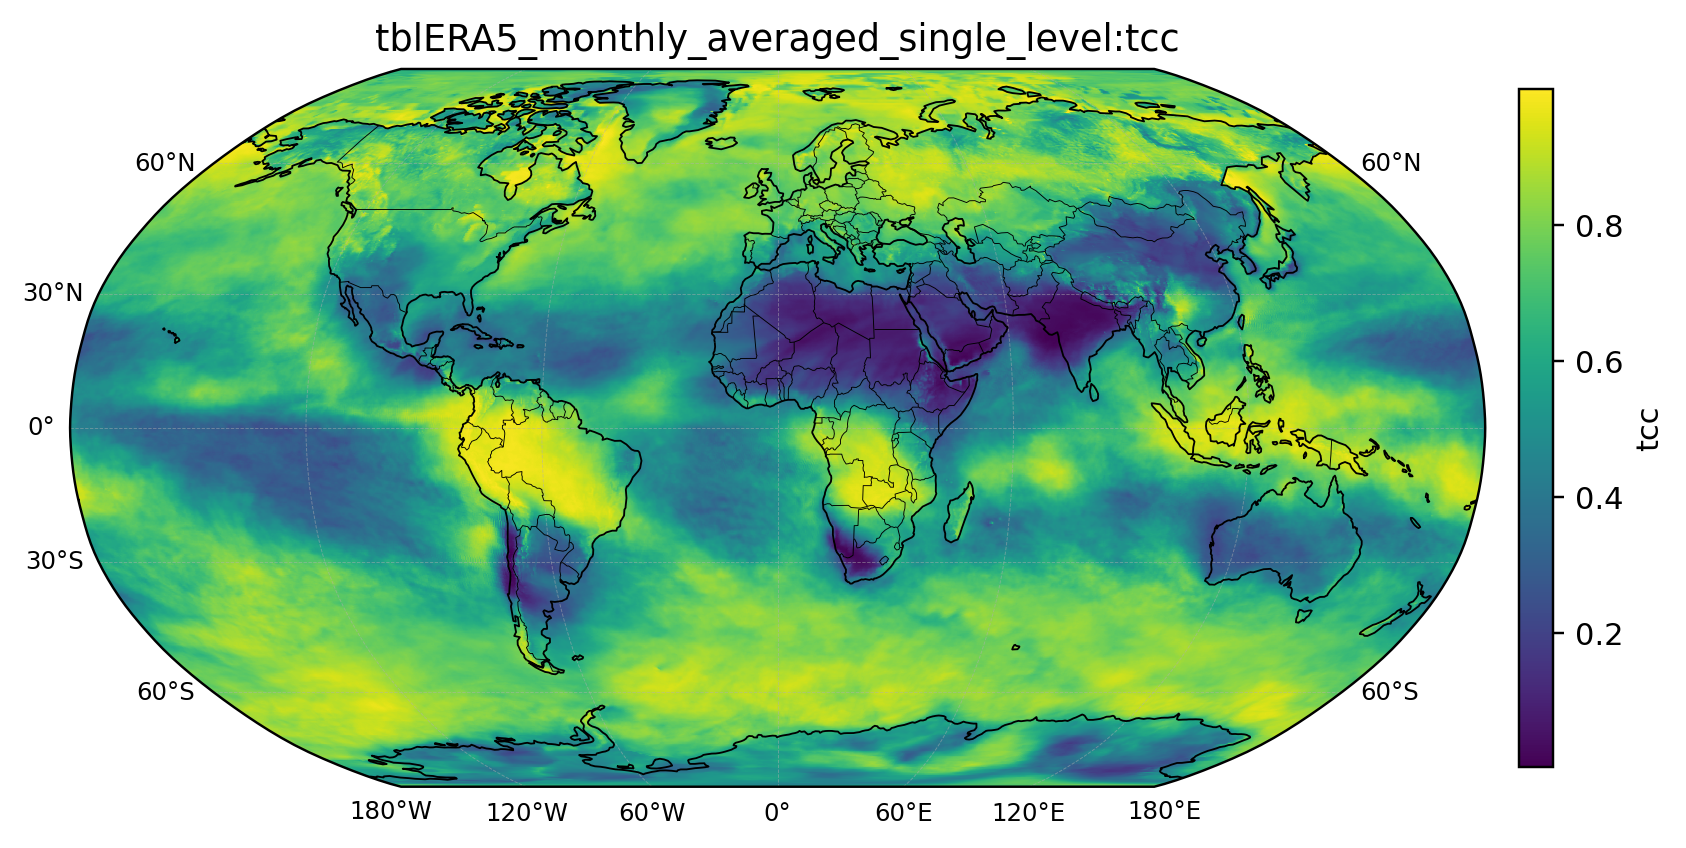
\includegraphics[width=\linewidth]{figures/tcc.png}
  \caption{Visualization workflow vignette. From a natural-language request, CMAP Agent generates a global map visualization of total cloud cover (tcc) for December 1945 from the ERA5 Monthly Averaged Single Levels dataset. Colors indicate cloud fraction, with coastlines and political boundaries overlaid for geographic context. The figure illustrates the agent’s ability to resolve a dataset/variable, retrieve the required subset, and produce a georeferenced map artifact that is returned as a downloadable figure file in a standard cartographic projection (Robinson)}
  \label{fig:vin_viz}
\end{figure}